\chapter{Systemarkitektur - Hardware}
\section{BDD}
\subsection{BDD diagrammer}
\begin{figure}[H]
	\centering
	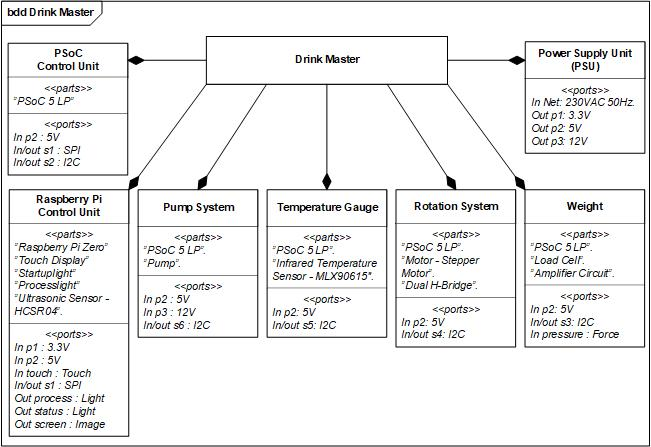
\includegraphics[width=1\textwidth, angle = 0]{Images/Hardwarearkitektur/BDD_System_Compact_JPEG.jpg}
	\caption{bdd for Drink master}
	\label{fig:bdd}
\end{figure}
\FloatBarrier

\begin{figure}[H]
	\centering
	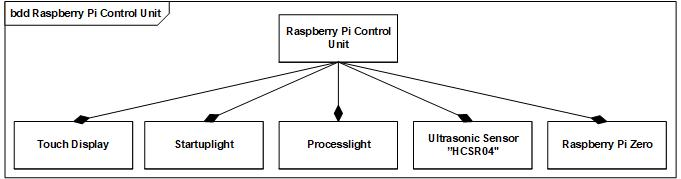
\includegraphics[width=1\textwidth, angle =0]{Images/Hardwarearkitektur/BDD_Raspberry_Pi_Control_Unit_JPEG.jpg}
	\caption{bdd for Raspberry Pi control unit}
	\label{fig:bdd_rasp}
\end{figure}
\FloatBarrier

\begin{figure}[H]
	\centering
	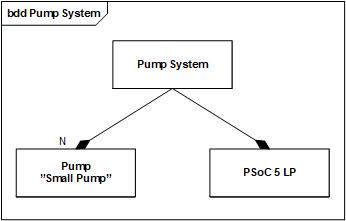
\includegraphics[width=0.7\textwidth, angle = 0]{Images/Hardwarearkitektur/BDD_Pump_System_JPEG.jpg}
	\caption{bdd for pump system}
	\label{fig:bdd_pump}
\end{figure}
\FloatBarrier

\begin{figure}[H]
	\centering
	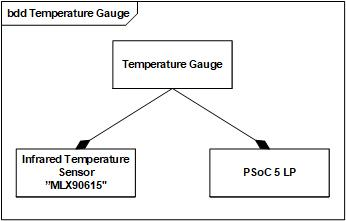
\includegraphics[width=0.7\textwidth, angle = 0]{Images/Hardwarearkitektur/BDD_Temperature_Gauge_JPEG.jpg}
	\caption{bdd for temperature gauge}
	\label{fig:bdd_temp}
\end{figure}
\FloatBarrier

\begin{figure}[H]
	\centering
	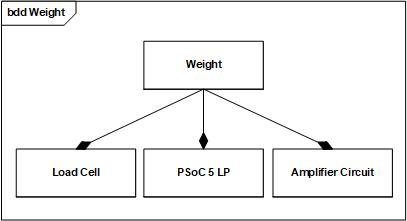
\includegraphics[width=0.7\textwidth, angle = 0]{Images/Hardwarearkitektur/BDD_Weight_JPEG.jpg}
	\caption{bdd for weight}
	\label{fig:bdd_weight}
\end{figure}
\FloatBarrier

\begin{figure}[H]
	\centering
	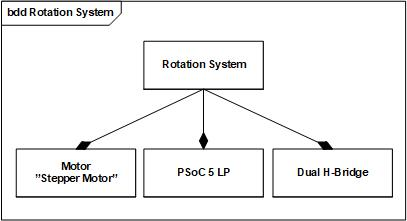
\includegraphics[width=0.7\textwidth, angle = 0]{Images/Hardwarearkitektur/BDD_Rotation_System_JPEG.jpg}
	\caption{bdd for rotaltion system}
	\label{fig:bdd_rotaltion}
\end{figure}
\FloatBarrier

\subsection{BDD beskrivelse}

\begin{table}[H] 
	\centering 
	\begin{tabular}{|p{3.5cm}|p{7cm}|p{2.5cm}|}
		\hline
\textbf{Bloknavn} & \textbf{Blokbeskrivelse}  &  \textbf{Kommentar}  \\ \hline
Raspberry Pi control unit (SPI Master)   & [Raspberry Pi Zero] SPI Master-enhed. Er forbundet med et [Touch Display], som er brugerens tilgang til systemet.  Har en [Ultrasonic Sensor] til at registrere om en bruger er inden for maskinens rækkevidde. Yderligere består den også af nogle lys til at både indikere om detektion af bruger [Startuplight], og processtatus [Processlight]. Kommunikerer med PSoC I2C Master-enhed. &  \\ \hline
PSoC Control Unit (I2C Master) & PSoC Control Unit
(I2C Master)	I2C Master-enhed i form af en [PSoC 5 LP], som kommunikerer direkte med alle andre enheder. Danner et kommunikationsled mellem alle I2C Slaver og SPI Masteren.   &  \\ \hline
Pump System (I2C Slave)              & Består af en [PSoC 5 LP] samt en pumpe [Pump] der doserer en prædefineret mængde af væske, fra en flaske ned i et indsat krus, som skal mixes i den valgte drink.                       &  \\ \hline
Temperature Gauge (I2C Slave) & Består af en [PSoC 5 LP] samt en [Infrared Temperature Sensor] til detektering af temperatur på flasker.  &  \\ \hline
PSU               & En strømforsyning som leverer de forskellige spændinger som systemet har brug for.                                                                               &  \\  \hline
Weight (I2C Slave)            & Et vægtsystem til at registrere indsat krus, og om væske er påfyldt kruset. Består af en [PSoC 5 LP], [Load Cell] til at registrere vægt og et [Amplifier Circuit] til at forstærke denne registrering.     &  \\ \hline
Rotation System (I2C Slave)   & Består af en [PSoC 5 LP] og en [Motor] som styrer et hjul med flasker. En flaske, som skal bruges til en valgt drink bliver positioneret ovenover et indsat krus. En [Dual H-Bridge] lader PSoC’en styre motorens retning, hastighed og position.   &  \\ \hline
	\end{tabular}
	\caption{Blokbeskrivelse for figur \ref{fig:bdd} bdd Drink master}
	\label{tab:blokbeskrivelse}
\end{table}
\FloatBarrier
\newpage

\section{IBD}
\subsection{IBD diagrammer}

\begin{figure}[h]
	\centering
	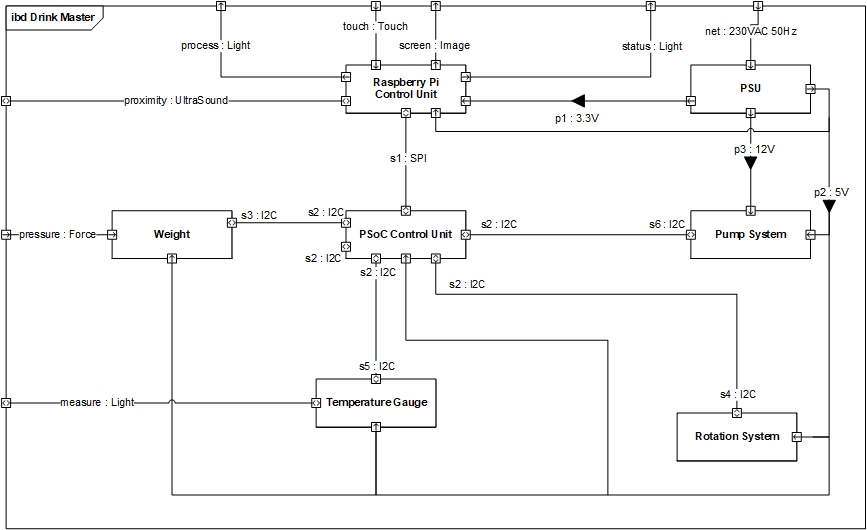
\includegraphics[width=1\textwidth]{Images/Hardwarearkitektur/IBD_System_JPEG.jpg}
	\caption{ibd for Drink master}
	\label{fig:ibd}
\end{figure}
\FloatBarrier

\begin{figure}[h]
	\centering
	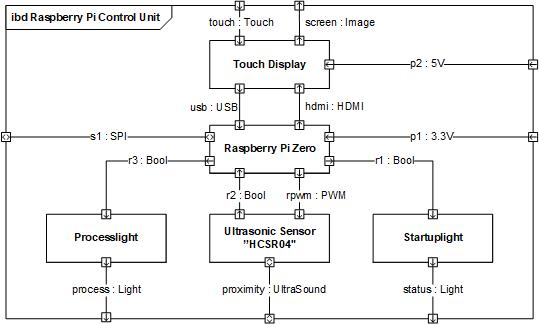
\includegraphics[width=1\textwidth]{Images/Hardwarearkitektur/IBD_Raspberry_Pi_Control_Unit_JPEG.jpg}
	\caption{ibd for Raspberry Pi control unit}
	\label{fig:ibd_rasp}
\end{figure}
\FloatBarrier

\begin{figure}[h]
	\centering
	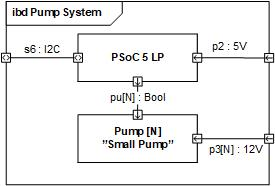
\includegraphics[width=0.5\textwidth]{Images/Hardwarearkitektur/IBD_Pump_System_JPEG.jpg}
	\caption{ibd for pump system}
	\label{fig:ibd_pump}
\end{figure}
\FloatBarrier

\begin{figure}[h]
	\centering
	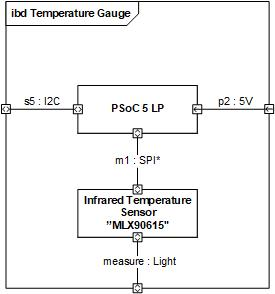
\includegraphics[width=0.5\textwidth]{Images/Hardwarearkitektur/IBD_Temperature_Gauge_JPEG.jpg}
	\caption{ibd for temperature gauge}
	\label{fig:ibd_temp}
\end{figure}
\FloatBarrier

\begin{figure}[h]
	\centering
	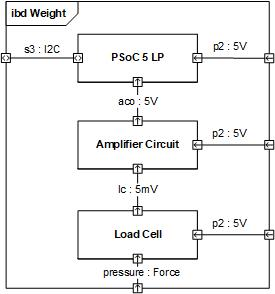
\includegraphics[width=0.5\textwidth]{Images/Hardwarearkitektur/IBD_Weight_JPEG.jpg}
	\caption{ibd for weight}
	\label{fig:ibd_weight}
\end{figure}
\FloatBarrier

\begin{figure}[h]
	\centering
	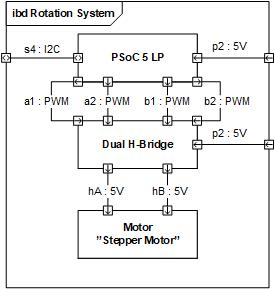
\includegraphics[width=0.5\textwidth]{Images/Hardwarearkitektur/IBD_Rotation_System_JPEG.jpg}
	\caption{ibd for rotation system}
	\label{fig:ibd_ratation}
\end{figure}
\FloatBarrier

\subsection{IBD beskrivelser}

\begin{table}[H] 
	\centering 
	\begin{tabular}{|p{2cm}|p{6cm}|p{2cm}|p{3cm}|}
		\hline
\textbf{Signal} & \textbf{Funktionsbeskrivelse}  & \textbf{Område} &  \textbf{Kommentar}  \\ \hline
P1 : 3.3V & Spændingsforsyning til Raspberry Pi Control Unit. & 3.13V-3.46V & Tolerance $\pm$ 5\%  \\ \hline
P2 : 5V & Spændingsforsyning til PSoC Control Unit: I2C Master, og tilhørende I2C Slaves. & 4.75V-5.25V & Tolerance $\pm$ 5\%  \\ \hline
P3 : 12V & Spændingsforsyning til Pumpe(r) i Pump System. & 11.4V-12.6V & Tolerance $\pm$ 5\% \\ \hline
S1 : SPI & SPI Kommunikation mellem Raspberry Pi Control Unit og PSoC Control Unit. & 0V-3.3V &  \\ \hline
S2 : I2C & I2C Kommunikation mellem PSoC Control Unit og PSoC Slaves. & 0V-5V &  \\ \hline 
S3 : I2C & I2C Kommunikation mellem Weight og PSoC Control Unit. & 0V-5V &  \\ \hline
S4 : I2C & I2C Kommunikation mellem Rotation System og PSoC Control Unit. & 0V-5V &  \\ \hline
S5 : I2C & I2C Kommunikation mellem Temperature Gauge og PSoC Control Unit. & 0V-5V &  \\ \hline
S6 : I2C & I2C Kommunikation mellem Pump System og PSoC Control Unit. & 0V-5V &  \\ \hline
Process : Light & Lys som indikerer om maskinen er færdig med at lave en drink. & \cellcolor{gray} &  \\ \hline
Status : Light & Lys som indikerer om maskinen har detekteret en bruger. & \cellcolor{gray} &  \\ \hline
Touch : Touch & Touch Display input fra bruger. & \cellcolor{gray} &  \\ \hline
Screen : Image & Touch Display billede, som viser et GUI. & \cellcolor{gray} &  \\ \hline
Proximity : UltraSound & Ultralydssignal som detekterer bruger. & \cellcolor{gray} &  \\ \hline
Pressure : Force & Vægt input, til registrering af krus og påfyldt væske. & \cellcolor{gray} &  \\ \hline
Measure : Light & Infrarødt lys til detektering af flasketemperatur. & \cellcolor{gray} &  \\ \hline
	\end{tabular}
	\caption{Signalbeskrivelse for figur \ref{fig:ibd} ibd Drink master}
	\label{tab:signalbeskrivelse}
\end{table}
\FloatBarrier

\begin{table}[H] 
	\centering 
	\begin{tabular}{|p{2cm}|p{6cm}|p{2cm}|p{3cm}|}
		\hline
\textbf{Signal} & \textbf{Funktionsbeskrivelse}  & \textbf{Område} &  \textbf{Kommentar}  \\ \hline
usb : USB & USB kommunikation fra Touch Display til Raspberry Pi Zero. & \cellcolor{gray} &  \\ \hline
hdmi : HDMI & HDMI kommunikation fra Raspberry Pi Zero til Touch Display & \cellcolor{gray} &  \\ \hline
r1 : Bool & Togglesignal fra Raspberry Pi Zero til Processlight. & 0V-3.3V &  \\ \hline
r2 : Bool & Togglesignal fra Ultrasonic Sensor til Raspberry Pi. & 0V-3.3V & Signalets varighed i en HIGH state bruges til at definere afstand. \\ \hline
r3 : Bool & Togglesignal fra Raspberry Pi Zero til Startuplight. & 0V-3.3V &  \\ \hline 
rpwm : PWM & PWM signal fra Raspberry Pi Zero til Ultrasonic Sensor, til generering af Ultralyd. & 0V-3.3V & Er HIGH i 10µS for at generere Ultralyd. \\ \hline
	\end{tabular}
	\caption{Signalbeskrivelse for figur \ref{fig:ibd_rasp} idb Raspberry Pi control unit}
	\label{tab:signalbeskrivelse_rasp}
\end{table}
\FloatBarrier

\begin{table}[H] 
	\centering 
	\begin{tabular}{|p{2cm}|p{6cm}|p{2cm}|p{3cm}|}
		\hline
\textbf{Signal} & \textbf{Funktionsbeskrivelse}  & \textbf{Område} &  \textbf{Kommentar}  \\ \hline
pu[N] : Bool & Togglesignal fra PSoC til Pumpe. Styrer hvornår pumpen skal dosere. & 0V-5V & [N] = Number of bottles.  \\ \hline
	\end{tabular}
	\caption{Signalbeskrivelse for figur \ref{fig:ibd_pump} ibd pump system}
	\label{tab:signalbeskrivelse_pump}
\end{table}
\FloatBarrier

\begin{table}[H] 
	\centering 
	\begin{tabular}{|p{2cm}|p{6cm}|p{2cm}|p{3cm}|}
		\hline
\textbf{Signal} & \textbf{Funktionsbeskrivelse}  & \textbf{Område} &  \textbf{Kommentar}  \\ \hline
m1 : SPI* & SPI Kommunikation* fra Infrared Temperature Sensor til PSoC. & 0V-5V &  TBD* \\ \hline
	\end{tabular}
	\caption{Signalbeskrivelse for figur \ref{fig:ibd_temp} ibd Temperature Gauge}
	\label{tab:signalbeskrivelse_temp}
\end{table}
\FloatBarrier

\begin{table}[H] 
	\centering 
	\begin{tabular}{|p{2cm}|p{6cm}|p{2cm}|p{3cm}|}
		\hline
\textbf{Signal} & \textbf{Funktionsbeskrivelse}  & \textbf{Område} &  \textbf{Kommentar}  \\ \hline
lc : 5mV & Variabelt spændingssignal fra Load Cell til Amplifier Circuit. & 0V-5mV &  \\ \hline
aco : 5V & Forstærket ”lc” signal fra Amplifier Circuit til PsoC. & 0V-5V &  \\ \hline
	\end{tabular}
	\caption{Signalbeskrivelse for figur \ref{fig:ibd_weight} ibd weight}
	\label{tab:signalbeskrivelse_weight}
\end{table}
\FloatBarrier

\begin{table}[H] 
	\centering 
	\begin{tabular}{|p{2cm}|p{6cm}|p{2cm}|p{3cm}|}
		\hline
\textbf{Signal} & \textbf{Funktionsbeskrivelse}  & \textbf{Område} &  \textbf{Kommentar}  \\ \hline
a[1:2], b[1:2] : PWM & PWM Signal fra PSoC til Dual H-Bridge. Styrer retning, hastighed og position for Stepper Motor gennem Dual H-Bridge. & 0V-5V &  \\ \hline
hA, hB : 5.25V & Spændingsforsyning gennem Dual H-Bridge. Bestemmer Stepper Motorens fase polaritet. & $\pm$5V &  \\ \hline
	\end{tabular}
	\caption{Signalbeskrivelse for figur \ref{fig:ibd_ratation} ibd rotation system}
	\label{tab:signalbeskrivelse_rotation}
\end{table}
\FloatBarrier